\documentclass[11pt]{exam}

\usepackage{amsmath}
\usepackage{graphicx}
\usepackage{geometry}
\usepackage{etoolbox}
\BeforeBeginEnvironment{choices}{\par\nopagebreak\minipage{\linewidth}}
\AfterEndEnvironment{choices}{\endminipage}
\geometry{
a4paper,
total={185mm,257mm},
left=10mm,
top=25mm,
bottom=10mm
}

\begin{document}
\setlength{\voffset}{-0.5in}
\setlength{\headsep}{5pt}

\fbox{\fbox{\parbox{8cm}{\centering
\vspace{2mm}
Testat - Versuch E - Diffusion und Osmose 
\vspace{2mm}
}}}
\hspace{2mm}
\makebox[0.25\textwidth]{Name:\enspace\hrulefill} \hspace{5mm}
\makebox[0.2\textwidth]{Datum:\enspace\hrulefill}
\vspace{4mm}

\begin{questions}

\question Die Leitfähigkeit von 30 ml Salzlösung wird zu 15,0 \( \frac{\mu S}{cm} \) bestimmt. Diese Salzlösung wird nun mit destilliertem Wasser auf 90 ml aufgefüllt. Welche Leitfähigkeit wird nun gemessen?

\begin{choices}
	\choice 45,0 \( \frac{\mu S}{cm} \)
	\choice 1,5 \( \frac{\mu S}{cm} \)
	\choice 15,0 \( \frac{\mu S}{cm} \)
	\choice 60,0 \( \frac{\mu S}{cm} \)
	\choice 5,0 \( \frac{\mu S}{cm} \)
\end{choices}

\vspace{3mm}\question In folgender Abbildung sehen Sie zwei Kammern, die durch eine semipermeable Membran getrennt sind. In der linken Kammer befindet sich zu Beginn eine Zuckerlösung, in der rechten nur Wasser. Das Wasser kann die Membran ungehindert durchdringen, der Zucker nicht. Welche Abbildung zeigt den Gleichgewichtszustand, der sich nach einiger Zeit einstellt? 

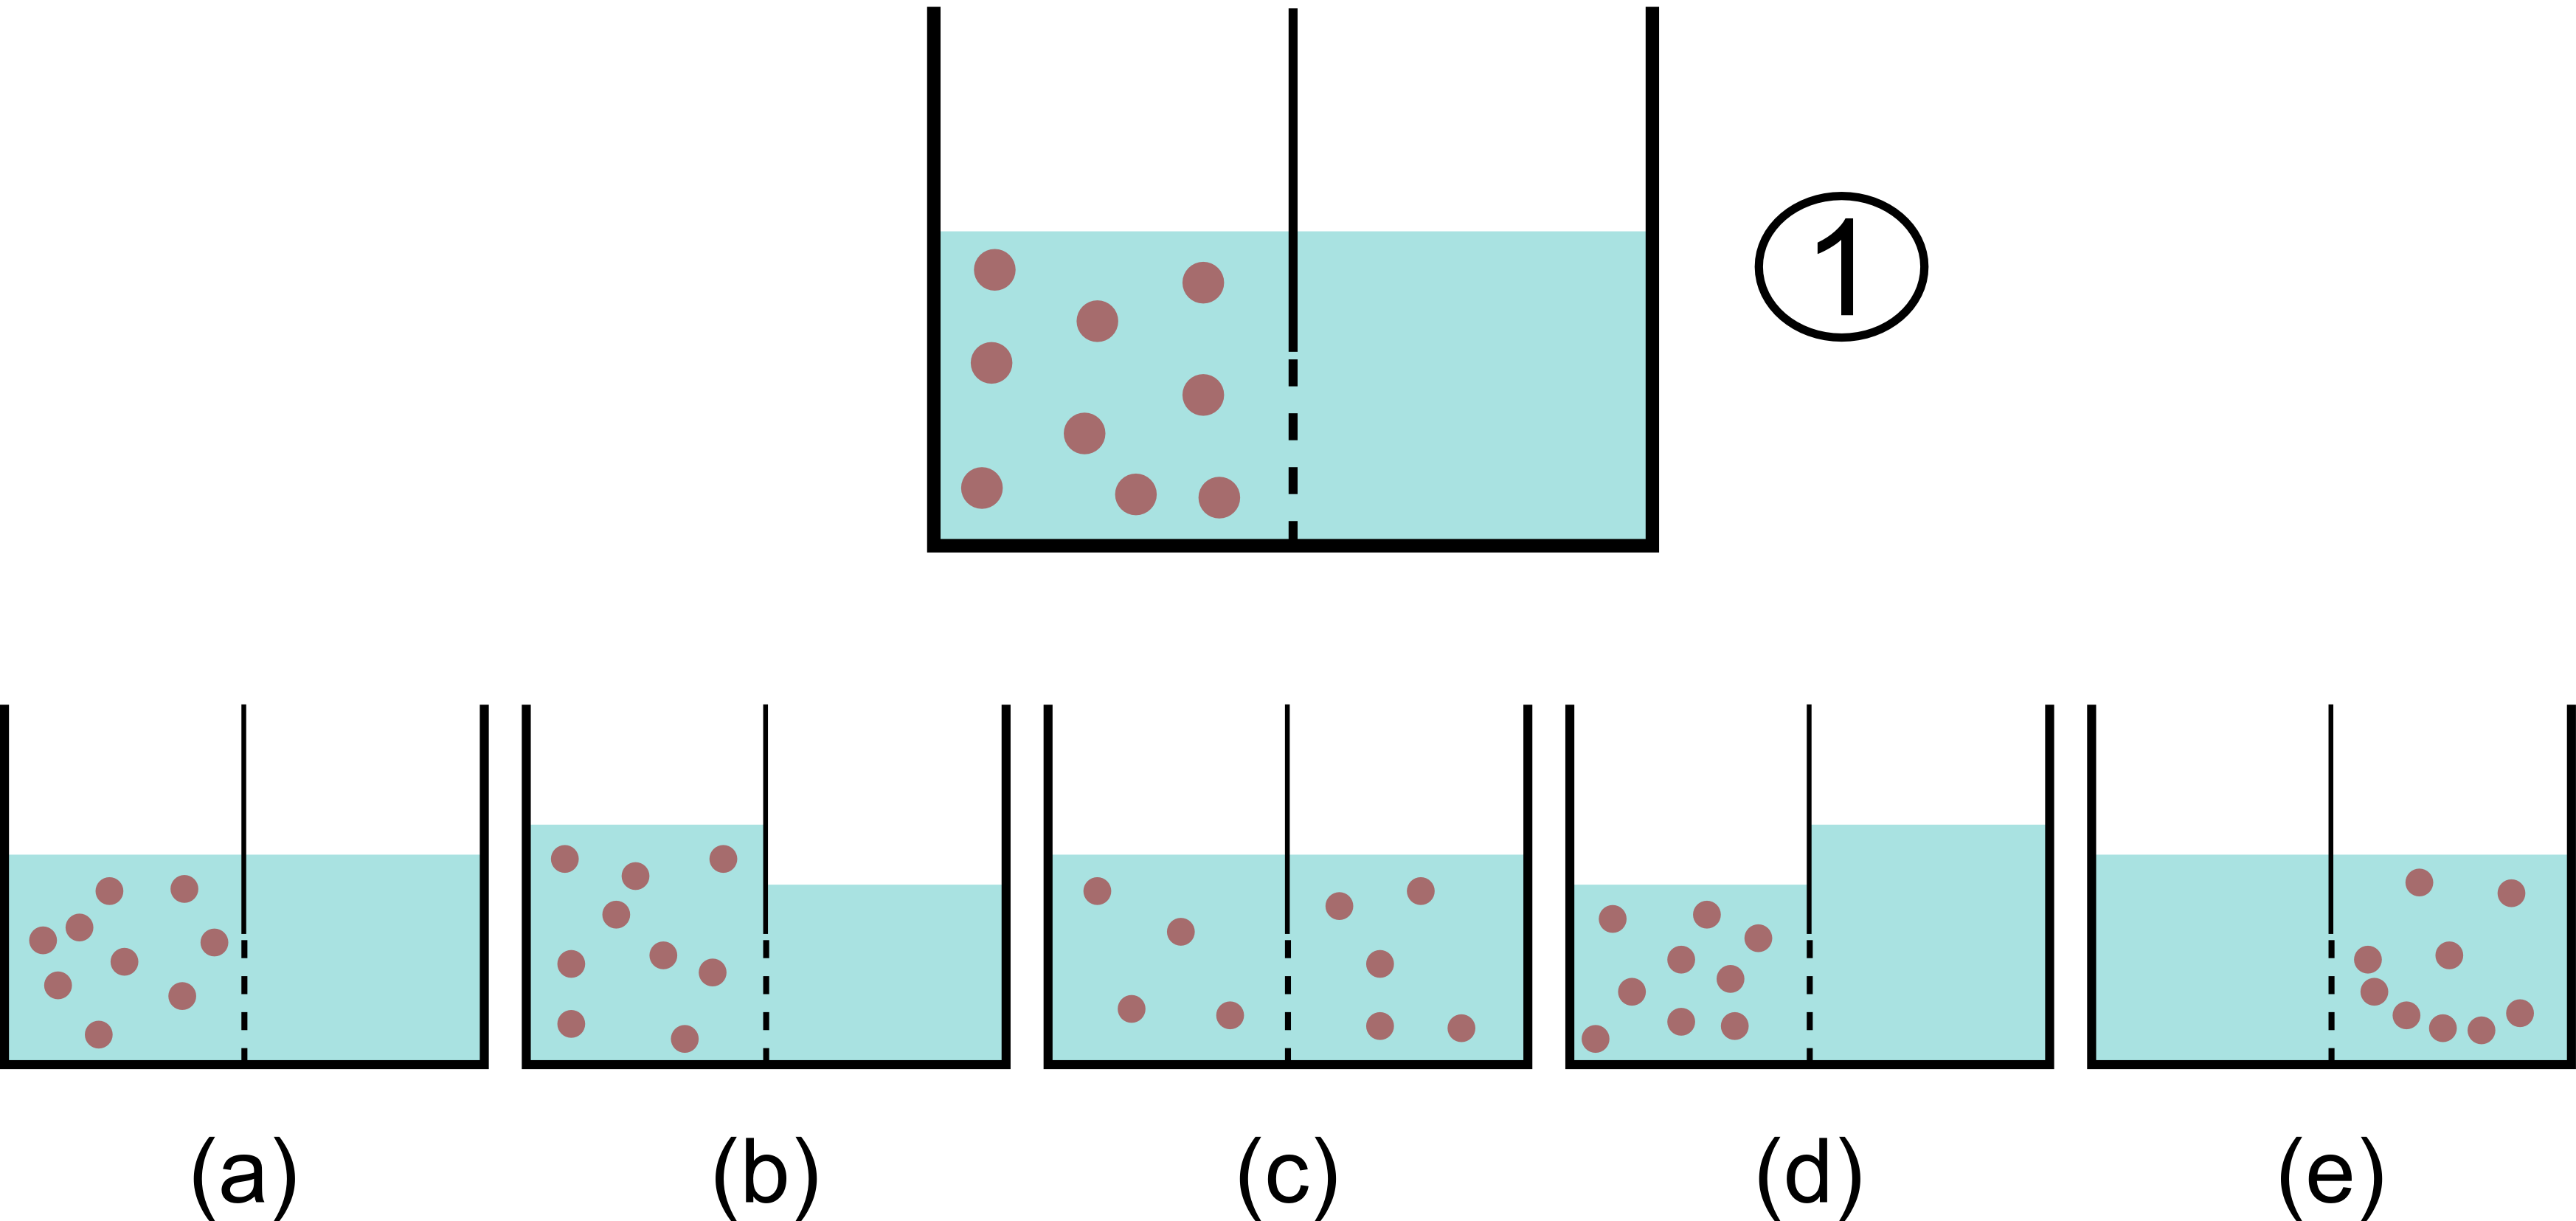
\includegraphics[width=0.4\textwidth]{images/Osmose.png}

\begin{choices}
	\choice e)
	\choice b)
	\choice c)
	\choice a)
	\choice d)
\end{choices}

\vspace{3mm}\question Wie ändert sich der Diffusionsfluss \( J \) durch eine kreisförmige Membran, wenn deren Durchmesser sich verdreifacht?

\begin{choices}
	\choice \( J \) nimmt um ein Drittel ab.
	\choice \( J \) verdoppelt sich.
	\choice \( J \) verdreifacht sich.
	\choice \( J \) ist unabhängig vom Durchmesser der Membran.
	\choice \( J \) verneunfacht sich.
\end{choices}

\vspace{3mm}\question Welche Aussage zur Osmose trifft zu?

\begin{choices}
	\choice ... steht mit dem Phänomen der Diffusion in keinem Zusammenhang
	\choice ... ist ein reversibler Prozess
	\choice ... lässt sich nicht direkt beobachten
	\choice ... hat in der Physiologie praktisch keine Bedeutung
	\choice ... ist ein irreversibler Prozess
\end{choices}

\vspace{3mm}\question Welche Einheit ist zur Angabe von Konzentrationen NICHT möglich?

\begin{choices}
	\choice \( l \cdot mol^{-1} \)
	\choice \( \frac{kmol}{l} \)
	\choice \( kmol \cdot m^{-3} \)
	\choice \( \frac{mol}{m^3} \)
	\choice \( mol \cdot cm^{-3} \)
\end{choices}

\vspace{3mm}\end{questions}

\end{document}
